\documentclass[UTF8]{article}
\usepackage{ctex}
\usepackage{geometry}
\geometry{a4paper, scale=0.8}
\usepackage{graphicx}
\usepackage{subfigure}
\usepackage{float}
\usepackage{bookmark}
\usepackage{fontspec}
\newfontfamily\jetbrains{JetBrains Mono}
\usepackage{listings}
\usepackage{color}
\lstset{
    breaklines,                                 % 自动将长的代码行换行排版
    extendedchars=false,                        % 解决代码跨页时,章节标题,页眉等汉字不显示的问题
    backgroundcolor=\color[rgb]{0.96,0.96,0.96},% 背景颜色
    keywordstyle=\color{blue}\bfseries,         % 关键字颜色
    identifierstyle=\color{black},              % 普通标识符颜色
    commentstyle=\color[rgb]{0,0.6,0},          % 注释颜色
    stringstyle=\color[rgb]{0.58,0,0.82},       % 字符串颜色
    showstringspaces=false,                     % 不显示字符串内的空格
    numbers=left,                               % 显示行号
    numberstyle=\tiny\jetbrains,                    % 设置数字字体
    basicstyle=\small\jetbrains,                    % 设置基本字体
    captionpos=t,                               % title在上方(在bottom即为b)
    frame=single,                               % 设置代码框形式
    rulecolor=\color[rgb]{0.8,0.8,0.8},         % 设置代码框颜色
}
\usepackage{enumitem}
\usepackage{hyperref}
\hypersetup{
    hypertex=true,
    colorlinks=true,
    linkcolor=black,
    anchorcolor=black,
    citecolor=black
}
\usepackage{caption}

\title{Verilog实验\ lab5实验报告}
\author{PB19071405\ 王昊元}
\date{2022 年 05 月 25 日}

\begin{document}
    \maketitle
    \section{实验目的}
    \begin{itemize}
        % \item 分别在CPU、GPU平台实现不同优化程度的矩阵乘法
        \item 通过实现矩阵乘法,学习并体会数据级并行的原理及效果
    \end{itemize}
    \section{实验要求}
    \begin{itemize}
        \item 在CPU平台实现基础矩阵乘法、AVX矩阵乘法、AVX分块矩阵乘法
        \item 在GPU平台实现基础矩阵乘法、分块矩阵乘法
    \end{itemize}
    \section{实验环境}
    \subsection*{CPU}
    \begin{itemize}
        \item MacBook Air(13-inch, 2017)
        \item macOS Big Sur 11.2.3
        \item 1.8 GHz Dual-Core Intel Core i5
        \item 8 GB 1600 MHz DDR3
    \end{itemize}
    \subsection*{GPU}
    \begin{itemize}
        \item 学校GPU集群
    \end{itemize}
    \section{实验核心实现}
    \subsection{CPU部分}
    \paragraph{基础矩阵乘法}
    使用三层循环,按照矩阵乘法定义实现即可。
    \begin{lstlisting}[language=c++]
void gemm_baseline(float *A, float *B, float *C, int N)
{
    for(int i = 0; i < N; i ++)
    {
        for(int j = 0; j < N; j++)
        {
            // C[i][j]
            int idx = idxs2idx(i, j, N);
            C[idx] = 0.0f;
            for(int k = 0; k < N; k++)
            {
                C[idx] += A[idxs2idx(i, k, N)] * B[idxs2idx(k, j, N)];
            }
        }
    }
    return;
}
    \end{lstlisting}
    \paragraph*{AVX矩阵乘法}
    在实现AVX矩阵乘法时,进行了一定的优化,具体算法为:
    用$A_{ij}$乘$B$的第$j$行的向量,结果加到$C$的第$i$行。
    \begin{lstlisting}[language=c++]
void gemm_avx(float *A, float *B, float *C, int N)
{
    __m256 vecA, vecB, vecC;
    // 先假设 n >= 3 即 N >= 8,向量不需要补0
    // 对于 n < 3的情况,因为会向量会初始化为0,所以不需要额外处理
    for(int i = 0; i < N; i++)
    {
        // init Matrix C
        for(int j = 0; j < N; j++)
        {
            // cout << idxs2idx(i, j, N) << endl;
            C[idxs2idx(i, j, N)] = 0.0f;
        }
        for(int j = 0; j < N; j++)
        {
            vecA = _mm256_set1_ps(A[idxs2idx(i, j, N)]);
            // 8 = 256 / 32
            for(int k = 0; k < N; k += 8)
            {
                vecB = _mm256_loadu_ps(B + idxs2idx(j, k, N));
                vecC = _mm256_loadu_ps(C + idxs2idx(i, k, N));
                vecC = _mm256_fmadd_ps(vecA, vecB, vecC);
                _mm256_storeu_ps(C + idxs2idx(i, k, N), vecC);
            }
        }
    }
    return;
}
    \end{lstlisting}
    \paragraph*{AVX分块矩阵乘法}
    在采用上述算法的基础(使用上述算法,可以避免矩阵转置,同时也能兼顾一定的局部性)上,进行矩阵分块运算,
    同时进行了一定的循环展开,在展开时,考虑数据IO的耗时,选择对$A_{ij}$进行展开,可以多次复用$B$的行向量。
    \begin{lstlisting}[language=c++]
void block(
    float *A, float *B, float *C,
    int N, int si, int sj, int sk,
    int block_size
)
{
    for(int i = si; i < si + block_size; i += UNROLL)
    {
        for(int j = sj; j < sj + block_size; j++)
        {
            // unroll a
            __m256 a[UNROLL];
            for(int x = 0; x < UNROLL; x++)
            {
                // A 的一列元素各自对应的向量
                a[x] = _mm256_set1_ps(A[idxs2idx(i + x, j, N)]);
            }
            for(int k = sk; k < sk + block_size; k += 8)
            {
                __m256 b;
                // b = [ B[j][k] ... B[j][k+7] ]
                b = _mm256_loadu_ps(B + idxs2idx(j, k, N));
                // unroll c
                __m256 c[UNROLL];
                for(int x = 0; x < UNROLL; x++)
                {
                    c[x] = _mm256_loadu_ps(C + idxs2idx(i + x, k, N));
                    c[x] = _mm256_fmadd_ps(a[x], b, c[x]);
                    _mm256_storeu_ps(C + idxs2idx(i + x, k, N), c[x]);
                }
            }
        }
    }
    return;
}
    \end{lstlisting}
    \subsection{GPU部分}
    \paragraph*{基础矩阵乘法}\mbox{}\\
    \begin{lstlisting}[language=c++]
__global__ void gemm_baseline(float *A, float *B, float *C, int N)
{
    int x = threadIdx.x + blockIdx.x * blockDim.x;
    int y = threadIdx.y + blockIdx.y * blockDim.y;
    if(x >= N || y >= N)
    {
        return;
    }
    C[x * N + y] = 0.0f;
    float *pa = A + x * N;
    float *pb = B + y;
    for(int i = 0; i < N; i++, pa++, pb += N)
    {
        C[x * N + y] += (*pa) * (*pb);
    }
    return;
}
    \end{lstlisting}
    \paragraph*{分块矩阵乘法}\mbox{}\\
    \begin{lstlisting}[language=c++]
__global__ void blocked_gemm_baseline(float *A, float *B, float *C, int N)
{
    int x = threadIdx.x + blockIdx.x * blockDim.x;
    int y = threadIdx.y + blockIdx.y * blockDim.y;
    if(x >= N || y >= N)
    {
        return;
    }
    
    int tmp_x = threadIdx.x;
    int tmp_y = threadIdx.y;
    int block_num = (N + blockDim.x - 1) / blockDim.x;

    // const int block_size = (1 << 3);
    const int block_size = size;

    __shared__ float blockA[block_size][block_size];
    __shared__ float blockB[block_size][block_size];
    int A_start = blockIdx.x * block_size * N;
    int B_start = blockIdx.y * block_size;
    int A_step = block_size;
    int B_step = block_size * N;

    // 使用tmp减少与数组的交互,提升速度
    // 矩阵规模为 2^13 时,可以从2s+提升到1s+
    float tmp = 0.0f;
    for(int i = 0; i < block_num; i++)
    {
        blockA[tmp_x][tmp_y] = A[A_start + i * A_step + tmp_x * N + tmp_y];
        blockB[tmp_x][tmp_y] = B[B_start + i * B_step + tmp_x * N + tmp_y];
        __syncthreads();
        for(int j = 0; j < blockDim.x; j++)
        {
            // C[x * N + y] += blockA[tmp_x][j] * blockB[j][tmp_y];
            tmp += blockA[tmp_x][j] * blockB[j][tmp_y];
        }
        __syncthreads();
    }
    C[x * N + y] = tmp;
}
    \end{lstlisting}
    \section{实验结果及分析}
    \subsection{CPU部分}
    \paragraph{结果展示}\mbox{}\\
    \begin{table}[H]
        \centering
        % \captionsetup{justification=centering}
        \caption{CPU上不同规模的三种矩阵乘法的时间(其中n为指数,分块大小为$2^6$)}
        \begin{tabular}{cccc}
            \hline
            n & 基础矩阵乘法/s & AVX矩阵乘法/s & AVX分块矩阵乘法/s \\
            \hline
            0 & 5e-06 & 2.1e-05 & 0.000433 \\
            1 & 3e-06 & 1.3e-05 & 0.000293 \\
            2 & 3e-06 & 1.4e-05 & 0.000284 \\
            3 & 7e-06 & 1.2e-05 & 4.2e-05 \\
            4 & 3.8e-05 & 1.6e-05 & 2.9e-05 \\
            5 & 0.000283 & 2.2e-05 & 3.5e-05 \\
            6 & 0.002573 & 6.6e-05 & 3.4e-05 \\
            7 & 0.018028 & 0.000239 & 0.000202 \\
            8 & 0.206072 & 0.001937 & 0.001514 \\
            9 & 2.04034 & 0.018129 & 0.01266 \\
            10 & 42.2682 & 0.322516 & 0.14661 \\
            \hline
        \end{tabular}
    \end{table}
    图\ref{cpu part}仅展示了n从0到6的三种矩阵乘法的时间变化趋势,
    因为n大于6时基础矩阵乘法时间较长,会导致图中n从0到6时的时间相对大小不明显。
    \begin{figure}[H]
        \centering
        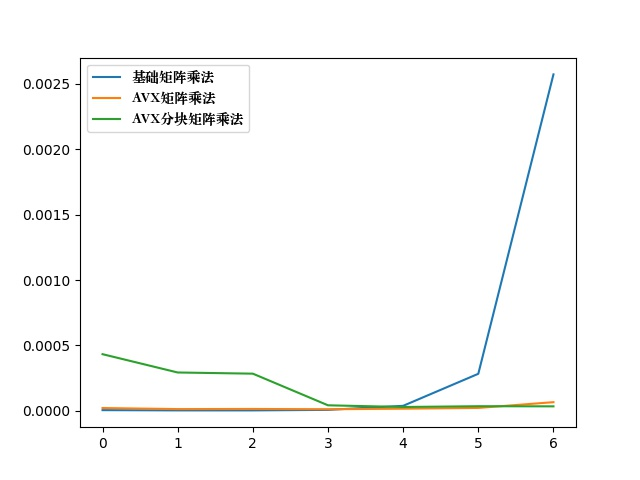
\includegraphics[width=0.7\textwidth]{./fig/cpu.jpg}
        \caption{n从0到6的三种矩阵乘法的时间趋势图}
        \label{cpu part}
    \end{figure}
    \begin{table}[H]
        \centering
        \caption{分块矩阵乘法不同块大小的时间(矩阵规模为$2^8$)}
        \begin{tabular}{ccccc}
            % \hline
            % 块大小 & 时间 \\
            % \hline
            % $2^3$ & 0.002098s \\
            % $2^4$ & 0.001625s \\
            % $2^5$ & 0.001632s \\
            % $2^6$ & 0.002396s \\
            % % $2^7$ & 0.001204s \\
            % \hline
            \hline
            块大小 & $2^3$ & $2^4$ & $2^5$ & $2^6$ \\
            \hline
            时间 & 0.002098s & 0.001625s & 0.001632s & 0.002396s \\
            \hline
        \end{tabular}
        \label{cpu blocksize influence}
    \end{table}
    \paragraph{结果分析}
    \begin{itemize}
        \item 从图\ref{cpu part}中可以看出,
        \begin{enumerate}
            \item 起初分块矩阵乘法明显慢于其他两种,这是由于分块矩阵每次运算的块的大小是一定的,所以对于较小的矩阵规模会做一些无用的工作。
            \item 在n较小时AVX矩阵乘法与基础矩阵乘法速度相差不大,且在n小于3(矩阵规模小于8)时,
            AVX矩阵乘法更慢,这是由于AVX每次执行是以向量为单位,而我在实现时使用{\jetbrains \_\_m256}存储大小为32bytes的float,
            一个向量存储8个单精度浮点数,所以当n大于3时,能发现AVX矩阵乘法明显快于基础矩阵乘法。
            \item 从图中数据发现即使当n较大时,分块矩阵乘法与AVX矩阵乘法相差无几,这是由于程序中的分块大小恰好为$2^6$
            (属于无意之举,分析时才发现),从原理上讲确实应相差无几,甚至在n为6时应该时间几乎一致才对,但比较数据会发现,
            分块矩阵乘法时间约为AVX矩阵乘法的一半,这是由于在分块矩阵乘法中进行了循环展开操作,一定程度上减少了数据IO的时间,
            比较n大于6时的数据,可以看到分块矩阵明显快于AVX矩阵,并且n越大效果更加明显。
        \end{enumerate}
        \item 从表\ref{cpu blocksize influence}中可以看到,随着分块大小的增大,矩阵乘法先变快后变慢,
        这可能是由于开始分块大小小于cache大小,随着分块越来越大,局部性利用得越来越好,速度越来越快,
        但慢慢分块大小超过了cache大小,计算分块时仍需要不断进行数据IO,且并行数越来越小,导致速度越来越慢。
        \item CPU平台上矩阵乘法的优化手段还有一些优化的细节或技巧,
        \begin{enumerate}
            \item 三层循环时,$j$(列索引)的循环放在外面,在矩阵较小时,可以利用cache来提高运算性能。
            \item 进行循环展开,同时对元素进行复用,可以大幅减少数据IO的次数,从而提高运算效率。
            \item 使用寄存器变量也可以在一定程度上提升矩阵乘法的性能。
            \item 使用指针代替数组索引可以在一定程度上提升性能。
        \end{enumerate}
    \end{itemize}
    \subsection{GPU部分}
    \paragraph{结果展示}\mbox{}\\
    \begin{table}[H]
        \centering
        \caption{GPU上不同规模的两种矩阵乘法的时间(其中n为指数,分块大小为$2^4$)}
        \begin{tabular}{ccc}
            \hline
            n & 基础矩阵乘法/s & 分块矩阵乘法/s \\
            \hline
            6 & 1.4400e-5 & 5.5680e-6 \\
            7 & 3.0016e-5 & 1.1999e-5 \\
            8 & 2.1897e-4 & 7.4143e-5 \\
            9 & 1.6277e-3 & 5.5228e-4 \\
            10 & 0.012601 & 4.2891e-3 \\
            11 & 0.10053 & 0.034157 \\
            12 & 0.62913 & 0.27016 \\
            13 & 5.14445 & 1.64694 \\
            \hline
        \end{tabular}
        \label{gpu}
    \end{table}
    表\ref{gpu}中,{\jetbrains blocksize}均为$8$,{\jetbrains gridsize}均为$\lceil\frac{N}{block size}\rceil$。
    \begin{table}[H]
        \centering
        \caption{GPU上不同{\jetbrains gridsize}、{\jetbrains blocksize}的两种矩阵乘法的时间}
        \begin{tabular}{cccc}
            \hline
            blocksize & gridsize & 基础矩阵乘法/ms & 分块矩阵乘法/ms \\
            \hline
            $2^3$ & $2^7$ & 12.602 & 4.2901 \\
            $2^4$ & $2^7$ & 24.327 & 8.8383 \\
            $2^5$ & $2^7$ & 53.835 & 27.590 \\
            $2^5$ & $2^6$ & 53.780 & 27.583 \\
            $2^5$ & $2^5$ & 53.805 & 27.582 \\
            \hline
        \end{tabular}
        \label{gpu size}
    \end{table}
    表\ref{gpu size}中,矩阵规模为$2^{10}$,分块大小为{\jetbrains blocksize}。
    \paragraph{结果分析}\mbox{}\\
    \begin{itemize}
        \item \begin{enumerate}
            \item 从表\ref{gpu}中可以看出,随着矩阵规模增大,矩阵乘法越来越慢,
            这是由于矩阵规模的增大带来的计算量增大,导致计算开销变多。
            \item 分块矩阵乘法明显快于基础矩阵乘法,这是由于分块矩阵乘法考虑了Cache,
            利用了数据的局部性,减少了数据IO的时间,从而提高了效率。
        \end{enumerate}
        \item 从表\ref{gpu size}中可以看出,随着blocksize的增大,矩阵乘法速度变慢,
        这可能是由于块越大,并行度越低,同时每个块的计算时间越长,最后导致矩阵乘法速度越来越慢。
        \item 从表\ref{gpu size}中可以看出,gridsize对矩阵乘法速度影响不大。
        \item 因为分块矩阵乘法需要约束分块大小与blocksize相同,故不单独分析分块大小对矩阵乘法的印象。
    \end{itemize}
    \section{实验总结}
    \begin{enumerate}
        \item 本次实验自己分别实现了CPU和GPU平台下的基础矩阵乘法和不同优化程度的矩阵乘法,
        切实体会到了数据级并行的效果。
        \item 在实验前的调研阶段让我大开眼界,对矩阵乘法方面的优化有了更深的了解。
    \end{enumerate}
\end{document}